{\bf BME154L - Spring 2012 - Exam \#2 Solutions}\hfill Name (Net ID):\underline{\hspace*{3.0in}}



\section{[50 points]}

\begin{center}
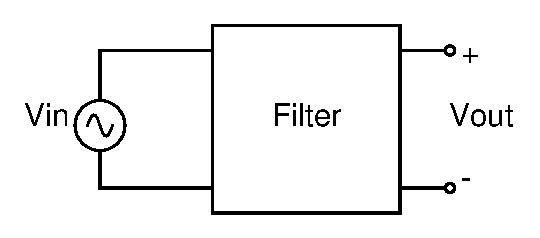
\includegraphics[width=0.5\linewidth]{filter/filter.eps}
\end{center}

You build the generalized circuit above in lab, and you measure the following $V_\textrm{out}$ signals for the specified $V_\textrm{in}$ signals (all measurements have $\pm$10\% tolerance on them):\footnote{It may help to think of these $V_\textrm{in}$ : $V_\textrm{out}$ pairs in terms of phasors.}

\begin{large}
\begin{center}
\begin{tabular}{|l|l|} \hline
$V_\textrm{in}$ (V) & $V_\textrm{out} (V)$ \\ \hline
15 $\sin(2000t)$ & 1.5 $\sin(2000t + \frac{\pi}{2})$ \\
10 $\sin(20000t + \frac{\pi}{2})$ & $\frac{10\sqrt{2}}{2}\sin(20000t + \frac{3\pi}{4})$ \\
2.5 $\cos(300000t)$ & 2.5 $\cos(300000t)$ \\
1.2 $\sin(4500000t)$ & $\frac{1.2\sqrt{2}}{2}\sin(4500000t - \frac{\pi}{4})$ \\
0.5 $\sin(45000000t + \frac{\pi}{2})$ & 0.05 $\sin(45000000t)$ \\ \hline
\end{tabular}
\end{center}
\end{large}

\begin{enumerate}
	\item Sketch Bode plots for the \underline{amplitude and phase} transfer functions for your filter.  Label everything important, including cut-off / resonance frequencies, if applicable.\footnote{I have only given you 5 discrete data points for your filter, but you can assume that all circuit behavior between these points is smooth and monotonic.} [15 points]
	\item You need to design a {\bf [ low-pass / high-pass / bandpass / bandstop ]} filter for these $V_\textrm{in}$ : $V_\textrm{out}$ relationships? Why? [5 points, choose one answer]
	\item Does your filter need to be active, or could you design a passive filter to achieve this $V_\textrm{in}$ : $V_\textrm{out}$  behavior? Why? [5 points]
	\item Draw the circuit diagram for your filter with all key components labeled with specified values.  If you are using op amps, then please specify their rail voltages. [10 points]
	\item What is the input impedance of your filter? [5 points]
	\item Design an amplifier for your filter output that can generate a maximum output voltage of $\pm$ 12 V and does not saturate (``rail'') for filter output voltages ($V_\textrm{out}$) as large as $\pm$ 2.5 V. Make sure that your amplifier does not corrupt the phase of the filter output ($V_\textrm{out}$).  Remember to consider the impedance relationship between your filter and your amplifier.  [10 points]
\end{enumerate}
